\chapter{Introducción}
\label{ch:introduction}

El \textit{skeleton} fue propuesto por Harry Blum en 1967 como una manera de capturar lo esencial de la forma de una figura biológica \cite{Blum:1967}. A diferencia de otros estímulos visuales como el color, la intensidad luminosa o el movimiento, Blum observó que el estudio de la forma habría estado sesgado por la geometría de las figuras. Las formas de figuras complejas, comunes en biología, casi no eran materia de estudio debido a la falta de herramientas para transformarlas en una combinación de componentes más simples. Blum postuló que la unión de los ejes medios, que más tarde sería llamada \textit{skeleton} \cite{hilitch1969linear}, podría haber sido la herramienta necesaria. Dada una figura, Blum define su \textit{skeleton} como una estructura delgada y centrada, geométrica y topológicamente expresiva.

\begin{figure}[ht]\centering
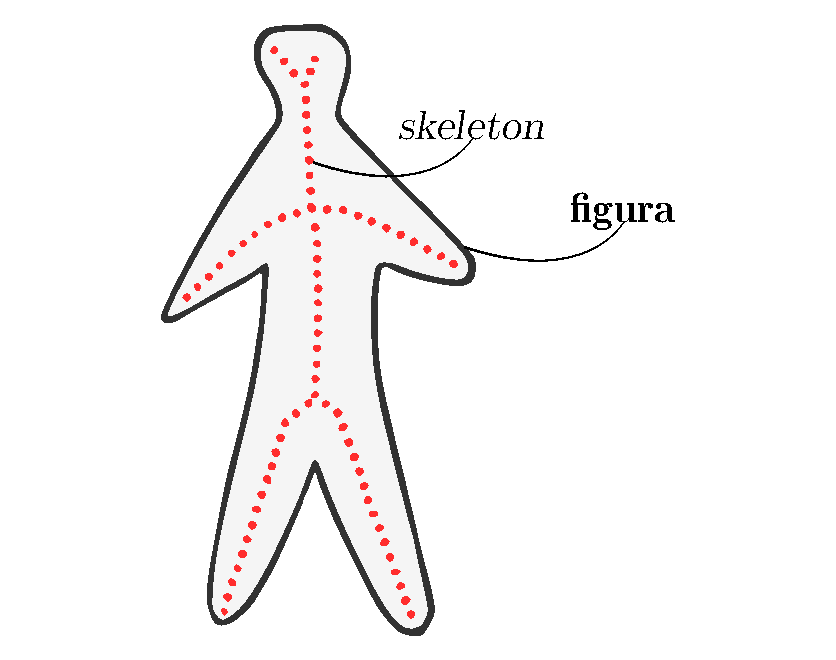
\includegraphics[width=0.5\linewidth]{images/blum}
\caption{Diagrama del \textit{skeleton} de una figura antropomórfica, como aparece en el artículo original de Blum \cite{Blum:1967}}.
\label{fig:blum}
\end{figure}

Cincuenta años mas tarde, el \textit{skeleton} de Blum se ha convertido en uno de los descriptores de figuras más usados \cite{sobiecki2013qualitative}. La operación de calcular el \textit{skeleton} juega un rol central en muchas aplicaciones que involucran la búsqueda, manipulación, análisis o compresión de figuras en el computador \cite{Saha2015}. La operación de calcular el \textit{skeleton} es también el foco de esta tesis. En principio, interesa responder la siguiente pregunta: ¿cuál es la mejor manera de llevar a cabo esta operación?

Existen al menos dos dificultades que impiden responder la pregunta anterior con facilidad.

\begin{enumerate}

\item Durante la extensa historia del \textit{skeleton} se han propuesto decenas de algoritmos para calcularlo. Siendo inviable comparar todos los métodos conocidos, es posible categorizarlos y seleccionar algoritmos representativos de cada clase. Sin embargo, las implementaciones de los algoritmos que calculan el \textit{skeleton} muy rara vez acompañan a su publicación \cite{sobiecki2014comparison}.

\item No existe un consenso para la definición del \textit{skeleton}. Es más, existen aplicaciones donde calcular un \textit{skeleton} demasiado ajustado a alguna definición puede ser perjudicial \cite{cornea2007curve}. Esto significa que cualquier comparación entre estos algoritmos debe plantearse en cuanto a las restricciones y objetivos de alguna aplicación en particular \cite{Saha2015}.

\end{enumerate}

En consideración con lo anterior, este trabajo de tesis se divide en dos partes. La primera parte consiste en implementar algoritmos representativos de las distintas maneras que se han propuesto para calcular el \textit{skeleton}. Luego viene la parte de comparar los \textit{skeletons} calculados. Los datos (las figuras cuyo \textit{skeleton} se quiere calcular) y la justificación para la comparación propuesta están ligados a una aplicación muy similar a la originalmente visionada por Blum. Interesa analizar el uso del \textit{skeleton} en la exploración y cuantificación de imágenes de figuras vivas microscópicas. En definitiva, la pregunta que busca responder esta tesis queda reformulada, a grandes rasgos, como sigue: ¿Qué clase de algoritmos para calcular el \textit{skeleton} es mejor para ciertas aplicaciones de biología?

El resto de este capítulo introductorio busca precisar lo señalado hasta este punto. Se revisan distintas maneras de definir y calcular el \textit{skeleton} de figuras 2D y 3D. Se detallan las propiedades del \textit{skeleton} de acuerdo a la literatura, dando ejemplos de aplicaciones donde satisfacer estas propiedades puede ser contraproducente. Finalmente, se  detalla la aplicación biológica del \textit{skeleton} que motiva este trabajo de tesis.

\section{Definiciones del \textit{skeleton}}

En la literatura es posible encontrar por lo menos cuatro definiciones formales para el \textit{skeleton} \cite{tagliasacchi20163d}. En esta sección se detallan las dos definiciones más populares \cite{cornea2005computing}, que al mismo tiempo son las más relevantes para este trabajo.



\subsection{Metáfora del incendio}
\label{ssec:grassfire}

La metáfora del incendio de Blum \cite{Blum:1967} dice que el \textit{skeleton} de un objeto se puede obtener encendiéndole fuego a toda su frontera simultáneamente. Luego, se asume que los frentes de llamas se propagan a una velocidad constante hacia el interior del objeto. Una vez que el fuego ha alcanzado todo el objeto, el \textit{skeleton} queda formado en los lugares donde dos frentes distintos se encontraron. En otras palabras, el \textit{skeleton} corresponde a los puntos de extinción, donde el fuego no pudo seguir avanzando por haberse encontrado consigo mismo. Estos puntos se conocen hoy en día como \textit{puntos de choque} \cite{leymarie2003three}. La Figura \ref{fig:horseonfire} ilustra esta definición.
\\\\
\begin{figure}[ht]\centering
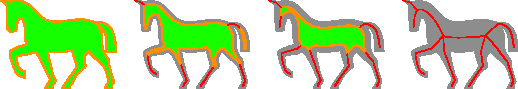
\includegraphics[width=0.9\linewidth]{images/horseonfire}
\caption{Progresión del fuego de la pradera en una imagen 2D}.
\label{fig:horseonfire}
\end{figure}

En este trabajo de tesis se implementaron dos algoritmos basados en esta definición. Estos son el algoritmo de adelgazamiento del Capítulo \ref{ch:palagyi} y el algoritmo de detección de singularidades del Capítulo \ref{ch:siddiqi}.

\subsection{Discos y bolas maximales inscritos}

La Figura X muestra un ejemplo de cálculo del \textit{skeleton} de una figura 2D y de dos figuras 3D.

El algoritmo del Capítulo \ref{ch:arcelli} está basado en esta definición.

\subsection{El \textit{skeleton} curvilíneo y el \textit{skeleton} de superficie}

Según las definiciones anteriores, el \textit{skeleton} de una figura 2D está constituido por rectas y curvas 1D, mientras que el \textit{skeleton} de una figura 3D puede contener, además de curvas 1D, superficies 2D. Debido a esto, el \textit{skeleton} de una figura 3D suele denominarse \textit{skeleton de superficie}. El \textit{skeleton} de superficie preserva la geometría general de la figura original. Tomando ciertas consideraciones, la figura 3D original puede recuperarse íntegramente a partir de su \textit{skeleton} de superficie \cite{borgefors1999computing}.

Sin embargo, salvo en aplicaciones donde interesa comprimir o reconstruir las figuras 3D originales, el \textit{skeleton} de superficie no es de mucha utilidad práctica. Su estructura es difícil de manipular y la presencia de parches de superficie lo vuelve inadecuado para muchas aplicaciones \cite{huang2013l1}. El \textit{skeleton curvilíneo}, una simplificación del \textit{skeleton} de superficie formada exclusivamente por curvas 1D, es mucho más usado. 

En particular, el \textit{skeleton} curvilíneo es el \textit{skeleton} que se usa en la aplicación que motiva esta tesis. Por lo tanto, los algoritmos implementados extraen en realidad el \textit{skeleton} curvilíneo. En adelante, salvo cuando el contexto sugiera algo distinto, la palabra \textit{skeleton} se usará para referirse al \textit{skeleton} curvilíneo.

\section{Propiedades del \textit{skeleton}} \label{sec:skelprops}

Las definiciones de la sección anterior, junto con las demás de la literatura, son usualmente equivalentes en teoría; es decir, en conjunto sugieren la existencia de un \textit{skeleton} formal para una figura. Sin embargo, llevar las definiciones a la práctica significa crear algoritmos fundamentalmente distintos entre sí. Como se comprobará a lo largo de esta tesis, incluso dos algoritmos que adopten la misma definición como punto de partida pueden producir \textit{skeletons} muy diferentes.

Se llega a la conclusión de que la definición de \textit{skeleton} no es muy útil para verificar el resultado de un algoritmo. Debido a esto, se han definido ciertas propiedades que un \textit{skeleton} debería satisfacer. Algoritmos diferentes satisfacen estas propiedades en distinta medida. Al mismo tiempo, aplicaciones diferentes favorecen algunas propiedades por sobre otras. Las propiedades más comúnmente encontradas \cite{cornea2007curve,tagliasacchi2012mean} se detallan a continuación.

Por otro lado, en contraste con el \textit{skeleton} de superficie, no existe una definición formal para el \textit{skeleton} curvilíneo \cite{reniers2008computing}.

\subsection{Homotopía}

La propiedad más básica.

\subsection{Centralidad}

El \textit{skeleton} debe estar centrado en la figura original.

\subsection{Delgadez}

El \textit{skeleton} de una figura de $n$ dimensiones debe ser una figura cuyas partes tienen a lo más $n-1$ dimensiones. El \textit{skeleton} se puede definir para un número de dimensiones arbitrario \cite{Lieutier20041029}, pero para esta tesis, puesto que concierne figuras representadas visualmente en el computador, $n$ vale 2 o 3. Entonces, el \textit{skeleton} de una figura 2D es una unión de curvas y el \textit{skeleton} de una figura 3D puede estar formado por curvas y parches de superficie.

\subsection{Suavidad}

teresa el surface
-- solo nos interesa el surface

Surface skeleton y curve skeleton

Hay dos formas de representar figuras en el computador, ambas igual de buenas.

\section{Clases de algoritmos}

La clasificación fue obtenida de \cite{tagliasacchi20163d}, por ser la más reciente y completa.

\subsection{Algoritmos de adelgazamiento topológico}

Los algoritmos de esta categoría entregan directamente el \textit{skeleton} curvilíneo.

\subsection{Algoritmos basados en distancia}

Los algoritmos de esta categoría buscan singularidades en algún campo definido para la imagen. Este campo depende de la distancia de cada elemento de la figura al borde de esta. El \textit{skeleton} es formado en los extremos de este campo.

Existen dos enfoques para calcular el \textit{skeleton}:

\begin{enumerate}
\item Calcular el \textit{skeleton} curvilíneo directamente, a partir de operaciones globales como la divergencia del campo (que es exactamente lo que hace el algoritmo del Capítulo \ref{ch:siddiqi}).
\item Calcular primero el \textit{skeleton} de superficie, y como segundo paso el \textit{skeleton} curvilíneo a partir de él (que es lo que hace el algoritmo del capítulo \ref{ch:arcelli}).
\end{enumerate}

En principio, los algoritmos del segundo enfoque deberían calcular un \textit{skeleton} más centrado. En ellos, el \textit{skeleton} final se calcula a partir del \textit{skeleton} de superficie, una figura centrada en la original.

\subsection{Algoritmos de proyección}

No fueron considerados.

\section{Estructura de esta tesis}

Cada uno de los próximos cuatro capítulos detalla un algoritmo de extracción de \textit{skeleton} implementado. Además de sus fundamentos teóricos, se describen los pormenores enfrentados durante cada implementación. Estos algoritmos fueron programados en el lenguaje MATLAB. Por completitud se incluye en el \autoref{ch:au} una descripción del algoritmo de contracción de mallas implementado en SCIAN-Lab para un trabajo anterior.

El foco de esta tesis es comprender, implementar y comparar algoritmos que extraen el \textit{skeleton} de datos 3D. Sin embargo, a lo largo de los capítulos posteriores el lector se encontrará también con definiciones y particularidades para el caso 2D. Esto porque, a juicio y por experiencia de quien escribe, en casi cualquier contexto imaginable el caso bidimensional resulta sustancialmente más accesible para el entendimiento humano comparado con el tridimensional. Comprender un concepto en el universo 2D, sienta las bases intuitivas para llevarlo más fácilmente a 3D. Cabe señalar que, fiel a lo anterior, cada algoritmo fue implementado primero en su versión 2D.
